\chapter{Methods}
\label{chapter:methods}

This chapter provides an overview of the fundamental methodological aspects considered for this study. Using an inductive approach, this research drew on an ethnographic methodological approach in which I constantly moved between online and offline mediums. Section \ref{sec:ethnography} presents an overview of ethnography and virtual ethnography, a discussion of the adequacy of this methodological approach for this study, and an overview of the fundamental aspects tackled in its application. Subsequently, the multi-modal character regarding data collection and generation --- combining participant observation, semi-structured qualitative interviews and documentary analysis --- is discussed in section \ref{sec:data-collection}. For each of these approaches, an overview of the type of data collected or generated, the sampling strategies, specific sources of partiality, as well as how these different modes were combined, is provided. Finally, section \ref{par:ethical-gen} discusses the main ethical considerations addressed during the course of this study.

\section{Methodological approach: an ethnographic perspective}
\label{sec:ethnography}

On the basis of the nature of the research questions presented in section \ref{subsubsec:state-art:drupal:case-study}, it was concluded that this study required an inductive approach --- assuming from the beginning that the main topics would emerge from the process of data analysis, rather than the other way around --- while aiming to understand the topics studied from inside the community. To this end, an ethnographic methodological approach was considered most suitable since it highlights the understanding of meanings from the point of view of Drupalistas due to the ``commitment to developing a deep understanding through participation and observation" \parencite[41]{hine2000virtualbook}.

These premises are congruent with calls to understand how effective forms of collective action and self-organisation are built in Commons-Based Peer Production from the perspectives of their participants. For example, as stated by \textcite[191]{troxler2014making} in his discussion about FabLabs framed within the area of Commons-Based Peer Production and the Third Industrial Revolution \parencite{rifkin2012third}, ``any relevant development in a peer-to-peer community will have to come from within. Study will have to be participative, not purely observational. Design has to be emergent, not prescriptive".

Ethnography is a methodological approach to study communities and cultures, dating back to the XIX century in the field of anthropology \parencite{hammersley2007ethnography}. This methodological approach would later be adopted in diverse fields --- such as sociology, cultural studies and history --- and there are various approaches to it. However, a set of characteristics are commonly shared by all these approaches \parencite[3]{hammersley2007ethnography}:

\begin{itemize}
	\item ``People's actions and accounts are studied in everyday contexts, rather than under conditions created by the researcher --- such as in experimental setups or in highly structured interview situations.", referring to carrying out research ``in the field", as this research required. However, as it will be discussed in section \ref{subsec:field-site}, the study of large and global CBPP communities, such as Drupal, requires further consideration regarding the field site when comparing with more traditional ethnographic studies focussed on communities whose boundaries are more clearly defined.
	\item ``Data are gathered from a range of sources, including documentary evidence of various kinds, but participant observation and\slash or relatively informal conversations are usually the main ones.", embracing multi-modal approaches, as that taken for this study, while highlighting the relevance of participant observation.
	\item ``Data collection is, for the most part, relatively `unstructured', in two senses. First, it does not involve following through a fixed and detailed research design specified at the start. Second, the categories that are used for interpreting what people say or do are not built into the data collection process through the use of observation schedules or questionnaires. Instead, they are generated out of the process of data analysis.", as congruent with the inductive approach followed for this study, in which a ``bottom-up" approach to move from specific observations towards broader generalisations and theories was followed.
	\item ``The focus is usually on a few cases, generally fairly small-scale, perhaps a single
setting or group of people.", as in the case of this research, focussed on a single case with the aim of facilitating in-depth study.
	\item ``The analysis of data involves interpretation of the meanings, functions, and consequences of human actions and institutional practices, and how these are implicated in local, and perhaps also wider, contexts.", referring to placing the focus on qualitative data, and assuming that quantification and statistical analysis have a secondary role, if any, as in the case of this research.
\end{itemize}

Adopting an ethnographic methodological approach for the study of a large and global CBPP community implied, however, a constant consideration of relevant questions regarding the research design that is acknowledged as emergent. Over the next subsections, an overview of the most relevant aspects considered for this research are presented.

\subsection{The field site: virtual ethnography and the study of online and offline activities}
\label{subsec:field-site}

Due to the digital nature of the main object produced --- software --- and the size and global nature of the community, a large amount of the day-to-day activity in the community is, unsurprisingly, carried out through online media. For that reason, this study drew on virtual ethnography \parencite{hine2000virtualbook}, an online research method that adapts traditional ethnographic methods for the study of online communities and their cultures\footnote{Several approaches and terms, such as virtual ethnography, netnography and digital ethnography, exist and are under ongoing methodological discussion. However, it was beyond the scope of this study to enter this discussion --- see \textcite{caliandro2014} for an overview of the differences between some of these approaches and terms. Instead, this study took a pragmatic stand making use of the adaptation of traditional methods for the study of online and also offline activity in the community.}.

Nevertheless, the relevance that offline activities have in the community emerged from the beginning of the study and it was consequently concluded that this research required immersion and participation in both online and offline activities. This approach is congruent with that already taken in similar studies due to the relevance of both dimensions, as in the study of FLOSS communities and hacker culture of \textcite{coleman2013coding}, since it allows a breakdown of the traditional dualism when necessary for the research focus \parencite{orgad2005online}. Furthermore, the online\slash offline distinction emerged as blurred and continuous, rather than binary, in which I needed to constantly move between different media. The definition of contribution activity as the main unit of analysis (see section \ref{subsec:at-conceptualisation}) facilitated, however, a clearer distinction with respect to my immersion and participation in the community. Two main categories of contribution activities emerged for this research design: ``mostly-online" and ``mostly-offline". 

``Mostly-online" contribution activities refers to \textsl{those in which actions and operations, from an Activity Theory perspective, are mostly performed through an online medium}. For instance, in the development of \textit{core} or \textit{contributed} projects, most actions and operations are typically carried out through digital platforms. However, offline activities are interconnected with these contribution activities and play a relevant role. For example, local communities organise F2F events specifically intended to contribute back to the community and collaborate in physical spaces, intertwining ``mostly-online" and ``mostly-offline" activities. Hence, it was concluded that the study of ``mostly-online" contribution activities required participation through both online and offline media.

Similarly, ``mostly-offline" contribution activities are defined in this study as \textsl{those in which actions and operations, from an Activity Theory perspective, are mostly performed through an offline medium}. For example, a better understanding of how events are organised or what the dynamics are behind them required physical participation in them. Nevertheless, online participation was also necessary to better understand their organisational dynamics, since online activity was found to play a significant role in this. For example, the coordination of these events is facilitated through online platforms, such as Drupal.org, and online tools, such as Telegram and Whatsapp groups. For these reasons, the study of these activities also required immersion and participation in online media, representing yet another indicator of the multi-faceted nature of these activities.

Hence, the field site considered for this case study was the set of online and offline spaces\footnote{The specific spaces in which participant observation was carried out and the reasons for selection will be extensively discussed in section \ref{subsec:participant-observation}.} in which the day-to-day of the community unfolds, as presented in section \ref{sec:drupal-history}, for which participation entailed a continuous process of transition between the online/offline dimensions.

\subsection{Position as ethnographer}
\label{subsec:ethnographic-position}

An important aspect to consider for this study was my position as an ethnographer, which could be defined as that of insider research  or self-ethnography \parencite{brannick2007defense},  in which ``the researcher-author describes a cultural setting to which s/he has a `natural access', is an active participant, more or less on equal terms with other participants. The researcher then works and/or  lives  in  the  setting  and  then  uses  the  experiences,  knowledge  and access to empirical material for research purposes." \parencite[174]{alvesson2003methodology}. When I started this research, I was already an active member of the Drupal community and had been for over three and a half years. This previous experience proved valuable for more rapid access to the community: from a faster understanding of the indigenous meanings around the software and the community, to practicalities for entering the field site and gaining access to certain activities, such as the organisation of events or the maintenance of official projects in Drupal.org. It also facilitated the process of acquiring the necessary social and technical skills to avoid being considered a ``newbie": a key aspect in ethnographic research in both offline and online spaces. For instance, in the ethnographic research carried out by \textcite{sveinsdottir2008virtual} on the Massive Multiplayer Online Game ``Star Wars Galaxies" as part of her PhD thesis, she described how a substantial amount of time to improve her gaming skills was required in order to avoid exasperating other players thus facilitating interactions with them.

This previous experience came at the cost, however, of having to address several challenges related to the dynamics of insider research, such as role duality and preunderstanding \parencite[67-71]{brannick2007defense}. Regarding the former, for example, this materialised in role conflicts which, on occasions, could be a potential source of displacement from the community studied. These types of issues were tackled by means of establishing a constant process of negotiation, in which both of my roles --- as a researcher and Drupalista --- were under continuous review and self-reflection. Regarding the latter, this was experienced, for instance, in the way the research processes progressed. For example, instead of a process of immersion in the community --- as commonly followed in ethnographic approaches ---  in my case it required me to move from the closeness to the distance and back again \parencite{nielsen1993nearness}, a frequent dynamic experienced by researchers crossing the insider-outsider boundaries \parencite{kanuha2000being}. Overall, this entailed a continuous process of rigorous introspection and reflection of my own experiences, while also gaining understanding by putting myself in the place of other Drupalistas. A clear example of this occurred, for instance, when reflecting on the notion of contribution in the community. Since my previous experience within the Drupal community was mainly as a software developer and site builder, my initial notion of contribution before entering the field as researcher rather than as Drupalista was considerably ``code-centric\footnote{This notion was already introduced in section \ref{subsubsec:state-art:floss:academic-research} and it will be exhaustively examined in chapter \ref{identifyng-contribution:chapter}.}". As the research progressed, I realised the need for a wider understanding of contribution from perspectives of Drupalistas with different roles\footnote{Section \ref{par:roles} will provide further details on Drupal roles and how they were conceptualised in this study.} to mine. These realisations led, for example, to self-reflection with regard to contribution, and understanding it considering other Drupalistas' perspectives, as well as having an impact on the definition of strategies for data collection.

\subsection{Community membership}
\label{par:who-is-member}

Another question tackled from the beginning of this research was: ``Who can be considered as a member of the Drupal community?". 

With regard to the study of online activity, the initial approach followed in this study was a common one in the study of online communities: consider a Drupalista\footnote{Several words are used in the Drupal community to self-denote their members: ``Drupaler", ``Drupalist", ``Drupalista", etc. The noun suffix ``-ist" is employed for a person who (1) ``does an action or activity",  (2) ``who makes or produces something specified", (3) ``who specialises in an art, science or skill", (4) ``or who adheres or advocates for certain doctrine, system or code or behaviour" \parencite{merrian-ist2014}. The Latin suffix ``-ista" is one of the etymological origins of the suffix ``-ist" in English, and has remained without changes in several Romance languages such as Spanish, Portuguese, Italian and Catalan \parencite{wiktionary-ista-etimology}. As in the case of the selection of the term FLOSS in section \ref{subsec:state-art:floss}, the term composed by this suffix will be employed for the sake of reflecting inclusivity in meanings and uses. More specifically, the Latin version of the suffix has been chosen in order to reflect diversity.} anyone who has a user account on the main collaboration platform, since this can be seen as an indicator of their interest. However, as the study progressed, it became clear that it was necessary to narrow the scope of these initial criteria since members who carry out low or no interaction at all with the community were included in the term `Drupalista'.

To this end, during the first stage of data collection and analysis a minimum criteria was defined on the basis of the indigenous concept of ``not a spammer role". This concept is used in the community to distinguish those users with a minimum of activity at Drupal.org from those who simply create an account. The process is manually\footnote{Indeed, throughout the study a more complex set of roles within Drupal.org was defined (see \url{https://www.drupal.org/drupalorg/docs/user-accounts/user-roles-and-permissions}), and the processes were decentralised by including a vouching system to distribute trust between Drupal.org users.} reviewed by members of the community, and the guidelines for the criteria are defined on the main collaboration platform \parencite{drupal-not-spammer-role}:

\begin{figure}[H]
	\centering
	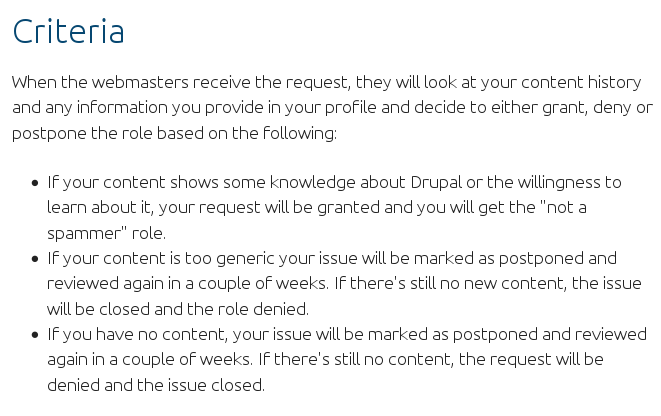
\includegraphics[scale=0.6]{img/quotes_replacement/drupal-not-spammer-role.png}
	\caption[Criteria for ``not a spammer role"]%
	{Criteria for ``not a spammer role". Retrieved \nth{6} October 2014, from \url{https://www.drupal.org/node/1887616}.}
	\label{not-spammer-quote}
\end{figure}

Although the technical specificities of the criteria are not publicly available, in several discussions with members of the Drupal.org webmasters group during the participant observation process, they explained that to fulfil the criteria, a significant amount of activity is required, showing that the user is real and not a robot\footnote{For privacy reasons, the technical specificities have been omitted as agreed with these Drupalistas.}.

Regarding the study of offline activities, the criteria for those who were considered part of the community was significantly more straightforward: any individuals present in the field site, discarding those who were not part of Drupal-related activity for the cases of events held in a public space (e.g. pub).

\subsection{Drupal roles: conceptualising division of labour within the Drupal community}
\label{par:roles}

A key concept for the research design of this study is that of the Drupal ``role". Within the community, this concept is understood as the different skills that members of the community have and the main tasks they perform while working with Drupal. This notion emerged as relevant from the beginning of the study. For example, some of the initial questions that I was asked while carrying out participant observation in F2F events attended for the first time were: ``What do you use Drupal for?" or ``Are you a developer or a themer?".

Table \ref{tab:drupal-roles} below illustrates the fundamental Drupal roles in the community, on the basis of a discussion within the community around the redesign of the main collaboration platform \parencite{drupal-roles-development}:

\begin{footnotesize}
\begin{longtable}{|p{3cm}||p{7cm}|p{3cm}|}
\hline
Drupal role                   & Description                                                                                                                                                                                        & Examples of Drupal-related technical skills                                                         \\ \hline \hline
System architect or devop              & Assemble and maintain infrastructures on which Drupal is deployed, manage the migration of data and content.                                                                          & MySQL, SSH, Solr, Apache                                                                             \\ \hline
Developer                     & Develop and test \textit{custom} modules according to Drupal's coding standards and best practices.                                                                                                         & PHP, MySQL                                                                                           \\ \hline
Themer or front-end developer  & Translate visual designs into code, develop \textit{custom} themes and \textit{custom} modules to implement the displays needed.                                                                           & CSS, Javascript, HTML                                                                                \\ \hline
Site builder                  & Install and configure modules to create site features. They have knowledge of theming and development, but mostly use Drupal through the administrative interface.                         & PHP, MySQL, Javascript                                                                               \\ \hline
Content Editor \& Manager     & Manage content and users on a Drupal site.                                                                                                                                                          & May not know many advanced functionalities of the Drupal administrative interface                \\ \hline
Design, UX                    & Possess an understanding of the capabilities of Drupal which helps to create designs which can be understood and implemented with their team.                                                    & Specialised in visual design, may not know HTML, CSS or JavaScript \\ \hline
Project Manager\slash Planner & Negotiate project plans with customers based on the understanding of the capabilities of Drupal. Understand best practices and communicate client needs in the language of Drupal to the team. & May not need any                                                                                     \\ \hline
Drupal Marketer               & Possess knowledge about Drupal's capabilities and applications and communicate them to clients and other audiences in ways best suited and understood by the client or audience.                & May not need any                                                                                     \\ \hline
\caption[List of Drupal roles.]{A non exhaustive list of the fundamental Drupal roles. Adapted from \textcite{drupal-roles-development}.}
\label{tab:drupal-roles}
\end{longtable}
\end{footnotesize}

The relevance of roles is also illustrated, for example, by their reflection in the artefacts employed for collaboration. For instance, figure \ref{roles_profile_dorg} displays how a field in the main user's profile at Drupal.org directly refers to this concept, and figure \ref{drupal-roles-tracks-dcon14} how it is reflected in the way tracks are organised in F2F events.

\begin{figure}[H]
	\centering
	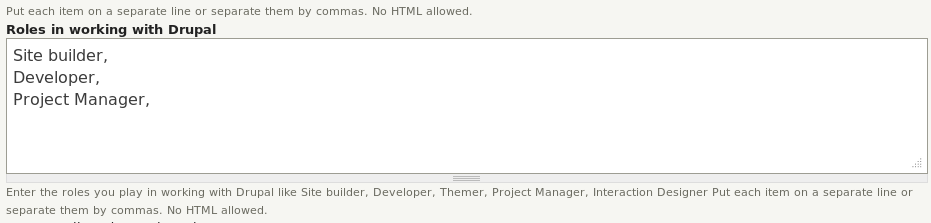
\includegraphics[scale=0.45]{img/roles_profile_dorg.png}
	\caption[Description of role field at Drupal.org's profile]%
    {Description of role field at Drupal.org's profile. Retrieved \nth{25} June 2014, from \url{https://www.drupal.org/user/}, under a CC BY-SA 2.0 license.}
	\label{roles_profile_dorg}
\end{figure}

\begin{figure}[H]
	\centering
	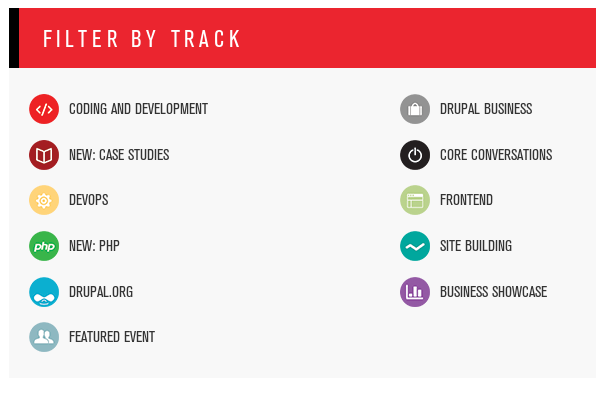
\includegraphics[scale=0.4]{img/drupal-roles-tracks-dcon14.png}
	\caption[Tracks at \textit{DrupalCon} Amsterdam 2014]%
    {Roles present in the tracks of \textit{DrupalCon} Amsterdam 2014. Retrieved \nth{24} September 2014, from \url{https://amsterdam2014.drupal.org/program/schedule/Tuesday}.}
	\label{drupal-roles-tracks-dcon14}
\end{figure}

As a result, the concept of roles was incorporated in this study and conceptualised as the ``division of labour" element from an Activity Theory perspective (see section \ref{subsec:at-conceptualisation}). Thus, this was considered while carrying out analysis and designing sampling strategies. It is essential to note that the notion of roles is not to be thought of as exclusive. Instead, the concept is better understood as comprehensive: Drupalistas usually identify themselves as having multiple roles, which is congruent with other studies on the Drupal community, in which limitations were found when assuming a single role while designing the research \parencite{nordin2013development}.

\section{Data collection}
\label{sec:data-collection}

This section provides an overview of the most relevant aspects regarding data collection and generation during this research. A multi-modal approach combining participant observation, documentary analysis and semi-structured qualitative interviews was adopted for data collection. The process drew on purposive sampling \parencite{palys2008purposive}, in which the collection of data was led by questions and emergent themes, and adapted for each thematic area and method\footnote{The subsequent subsections provide a more detailed explanation of how this was carried out.} to produce a relevant range of contexts that enabled the establishing of strategic and cross-contextual comparisons to build a well-founded argument \parencite[123-127]{mason2002qualitative}.

In congruence with the ethnographic methodological approach followed, data collection was relatively `unstructured' and the themes were generated from the data analysis rather than built into the process \parencite[3]{hammersley2007ethnography}. Data collection and content analysis informed each other, resulting in an overall process characterised by constant comparison and discovery in order to facilitate the emergence of concrete thematic areas \parencite{altheide1987reflections}. Also, sampling procedures were informed by theory and the themes explored.

Following the discussion presented in chapter \ref{sec:theoretical-frameworks} with regards to the study of self-organisational processes through the notion of contribution, two main thematic areas emerged and structured this study. Firstly, the notion of contribution in CBPP communities, which emerged during the initial stage of data collection and analysis, between November 2013 and October 2014. The initial main categories employed to pre-code and classify data are summarised in table \ref{main-categories-TA1}.

\begin{footnotesize}
\begin{longtable}{|p{3cm}||p{9cm}|}

\hline
Theme                                      & Description \\ \hline \hline
Governance and decision-making             & Governance and decision-making processes in the Drupal community, including activities of a diverse nature: coding, organisation of events and online community management among others. \\ \hline
Conflicts and tensions                     & Different controversies and tensions related to the organisation of the Drupal community. For example, the creation of a fork of Drupal, the relationships between the community and large corporations, and technical changes in the architecture provoking a potential expulsion of hobbyists among others. \\ \hline
Changes in the main collaboration platform & Evolution of Drupal.org and the ecosystem of sub-platforms around it. \\ \hline
Economic sustainability                    & Economic ecosystems around certain types of contribution, and the emergence of new initiatives. \\ \hline
Contribution                               & Contribution activities, including their differences, their organisational procedures and outcomes and motivations to contribute, among others. \\ \hline
\caption[Summary of the main categories for the first thematic area]{Summary of the main categories that emerged as part of the analysis for the first thematic area.}
\label{main-categories-TA1}
\end{longtable}
\end{footnotesize}

Nevertheless, after several major iterations the notion of contribution emerged as the core category, since it operated as a common thread for the remaining categories. Furthermore, this notion emerged as central, influencing the rest of the study: from fundamental aspects such as the selection of Activity Theory (see chapter \ref{sec:theoretical-frameworks}) as the main theoretical framework, to the decision to focus the study on the organisational dynamics of some of these contribution activities during subsequent stages.

The second thematic area referred to the self-organisational processes and dynamics that surround contribution activities in Commons-Based Peer Production communities, the data collection and analysis of which took place between October 2014 and November 2016. Key notions that emerged from the previous stage and considered as requiring further exploration were also incorporated into the study as part of this thematic area. For example, the ``mostly-online"/"mostly-offline" dimension and degree of formalisation were a fundamental part of the strategic sampling for activities to study.

A range of contribution activities was selected, considering these criteria. On one hand, for ``mostly-online" activities, the development of \textit{core}, \textit{contributed} and \textit{custom} projects was selected for study. The reason for this choice was based on the relevance these activities were shown to have in the day-to-day life of the community during the previous analytical stage, and the possibility of establishing cross-contextual analysis between them (e.g. in their peer-reviewing practices).  On the other hand, for ``mostly-offline" activities, the organisation of events --- local events, \textit{DrupalCamps} and \textit{DrupalCons} --- was selected for study. Similarly, this selection was based on relevance and the possibility of establishing cross-contextual analysis between differing self-organisational processes as well as those from the ``mostly-online" dimension. Tables \ref{project-chars} and \ref{f2f-events-chars} provide an overview of the activities whose organisational aspects were studied, together with the main identified characteristics.

    \begin{footnotesize}
    \begin{longtable}{p{3cm}||p{3cm}|p{3cm}|p{3cm}|}
    \cline{2-4}
& \textit{Core} projects & \textit{Contributed} projects & \textit{Custom} projects                                                 \\ \hline \hline
\multicolumn{1}{|p{3cm}||}{Description} & Official projects that form part of the default download of Drupal & Official projects that provide new functionalities that are not part of the core & Projects created for a particular use, case-specific for the site \\ \hline
\multicolumn{1}{|p{3cm}||}{Transition} & They might be excluded from core (inverse) & On occasions, they transit to become \textit{core}                                        & On occasions, they transit to become \textit{contributed}                \\ \hline
    \multicolumn{1}{|p{3cm}||}{Platforms availability}                              & Drupal.org & Drupal.org and external & External, if any                                                \\ \hline
    \multicolumn{1}{|p{3cm}||}{Amount in official collaboration platform}           & Tens & Thousands & Not applicable                                                  \\ \hline
    \multicolumn{1}{|p{3cm}||}{Degree of formalisation of peer reviewing processes} & High & Medium & Low                                                             \\ \hline
    %\end{tabular}
    \caption[Summary of the main characteristics of the Drupal projects studied]{Summary of the main characteristics of the Drupal projects studied as part of the analysis for the second thematic area.}
    \label{project-chars}
    \end{longtable}
    \end{footnotesize}



    \begin{footnotesize}
    \begin{longtable}{p{3cm}|p{3cm}|p{3cm}|p{3cm}|}
    \cline{2-4}
& Local events      & \textit{DrupalCamps}\footnote{See footnote \ref{fn-dev-days}.} & \textit{DrupalCons}         \\ \hline \hline
\multicolumn{1}{|p{3cm}||}{Organisers} & Local groups & Local groups, typically with help from other local communities within the regional and/or national scope & Drupal Association \\ \hline
\multicolumn{1}{|p{3cm}||}{Scope} & Local             & Regional and/or national & Global        \\ \hline
\multicolumn{1}{|p{3cm}||}{Frequency} & Typically monthly & Typically yearly & Yearly             \\ \hline
    \multicolumn{1}{|p{3cm}||}{Total number of events organised per year} & Hundreds          & Tens & 2 or 3             \\ \hline
    \multicolumn{1}{|p{3cm}||}{Number of attendees} & Tens            & Hundreds & Thousands          \\ \hline
    \multicolumn{1}{|p{3cm}||}{Typical cost of a ticket} & Usually free      & Tens of euros & Hundreds of euros  \\ \hline
    \multicolumn{1}{|p{3cm}||}{Typical duration} & Hours             & 2 or 3 days & 1 week             \\ \hline
    \multicolumn{1}{|p{3cm}||}{Degree of formalisation} & Low               & Medium & High               \\ \hline
    \caption[Summary of the main characteristics of the Drupal F2F events studied]{Summary of the main characteristics of the Drupal F2F events studied as part of the analysis for the second thematic area.}
    \label{f2f-events-chars}
    \end{longtable}
    \end{footnotesize}

The subsequent subsections provide an extensive discussion of the fundamental aspects regarding data collection for each method, comprising the types of data, details on how the purposive sampling was designed, the straddling between the online and offline dimension, and the integration with other methods. Finally, the section concludes with a brief overview of the strategies carried out to organise and store data.

\subsection{Participant observation}
\label{subsec:participant-observation}

Participant observation is a qualitative data collection method aiming to gain an in-depth understanding of the group studied through intensive involvement with it. Its relevance is highlighted by ethnographic approaches as those followed in this study. As discussed in section \ref{subsec:field-site}, this research required constant immersion and participation in the community in both online and offline spaces. This participant observation was carried out over three years: starting on \nth{22} November 2013 and concluding on \nth{24} November 2016. The main outcomes of this method were full field notes, which were systematically created in less than 24 hours after the participation in offline events as well as after relevant discussions or interactions through online media.

Regarding the online field site, there was constant engagement in diverse collaborative tasks carried out in the Drupal community in the spaces presented in section \ref{subsec:field-site}: joining and participating in discussion groups, developing and maintaining Drupal projects, creating documentation, participating in discussions via social networks and external platforms such as Meetup and interacting via IRC channels. The starting point was the main collaboration platform: Drupal.org. The ``Community\footnote{\url{https://drupal.org/community}, accessed on \nth{6} May 2014.}" section, for example, lists the different channels through which the community is officially present online, including working groups\footnote{\url{https://groups.drupal.org}, accessed on \nth{6} May 2014.}, a set of aggregated blog posts written by members of the community\footnote{\url{https://drupal.org/planet}, accessed on \nth{6} May 2014.}, mailing lists\footnote{\url{https://drupal.org/mailing-lists}, accessed on \nth{6} May 2014.}, forums\footnote{\url{https://drupal.org/forum}, accessed on \nth{6} May 2014.}, IRC channels\footnote{\url{https://drupal.org/irc}, accessed on \nth{6} May 2014.} or the website of the Drupal Association\footnote{\url{https://assoc.drupal.org}, accessed on \nth{6} May 2014.}.  All of these channels were considered part of the online field site for participant observation. For example, figure \ref{telegram_interaction} depicts an interaction via Drupal.org with a Drupalista who provided a patch in a \textit{contributed} project I maintain.

\begin{figure}[H]
    \centering
    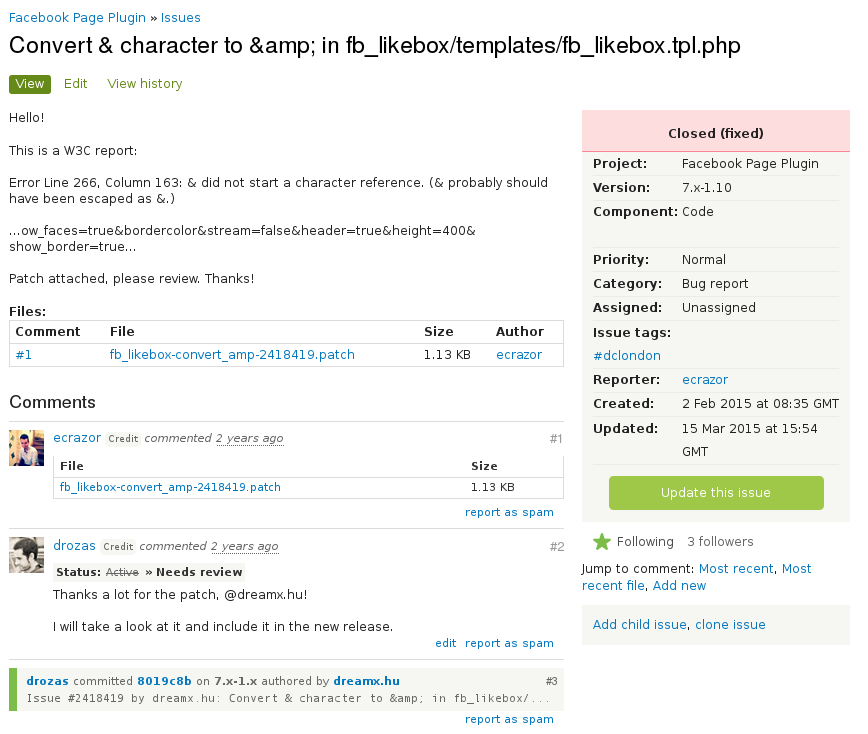
\includegraphics[scale=0.45]{img/tools/d_org_issue.png}
    \caption[Example of an interaction via Drupal.org]%
    {Example of an interaction via Drupal.org: a Drupalista nicknamed ``ecrazor" (previously nicknamed ``dreamx.hu") submitted a patch which I (``drozas") reviewed and committed into the project. Retrieved \nth{25} March 2015, from \url{https://www.drupal.org/node/2418419}.}
    \label{d_org_interaction}
\end{figure}

Furthermore, beyond these ``official" channels, several other online spaces emerged as relevant in the online medium as the study was being carried out. For example, the participation in private groups organised through Whatsapp or Telegram, external platforms such as Slack\footnote{See \url{https://slack.com}.} and StackExchange\footnote{See \url{http://drupal.stackexchange.com}.}, the interactions with Drupalistas via Twitter, and conversations via Skype and Google Hangout, to name but a few, became more relevant than originally expected. Figure \ref{telegram_interaction} depicts one of these private groups formed by Spanish Drupalistas attending \textit{DrupalCon} Barcelona 2015 to which I was invited.

\begin{figure}[H]
    \centering
    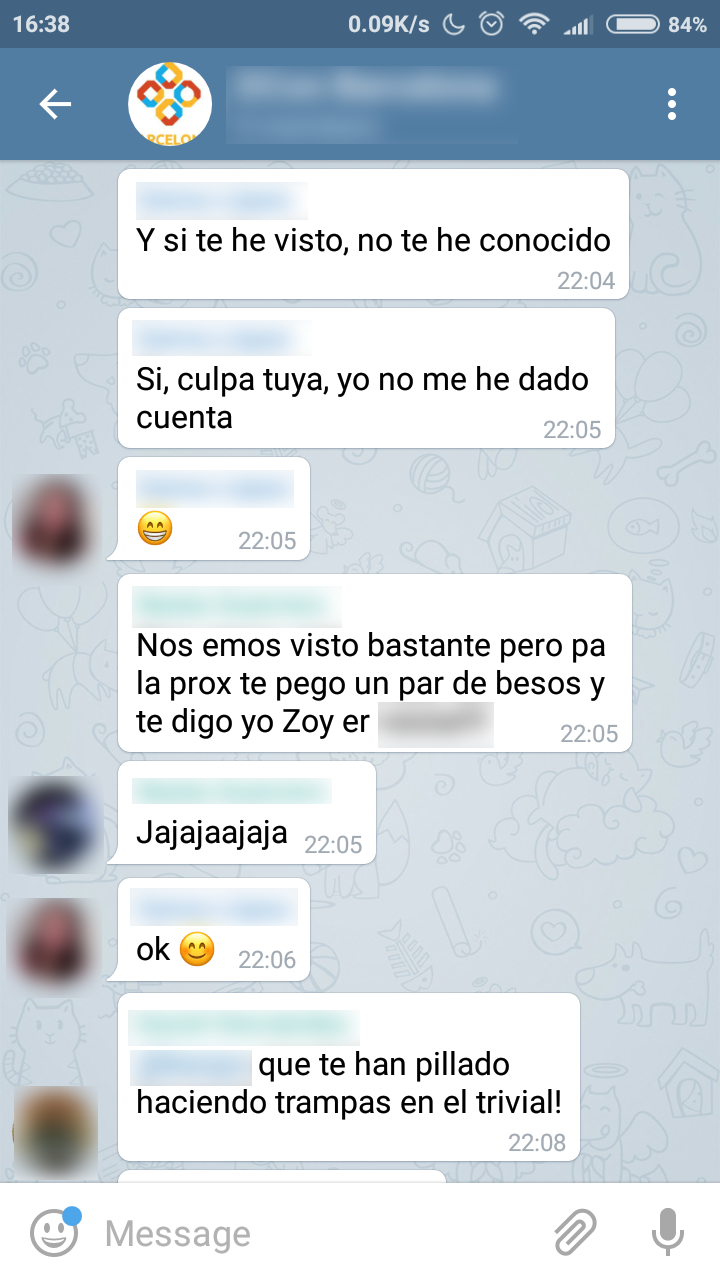
\includegraphics[scale=0.25]{img/tools/telegram_dcon.png}
    \caption[A private telegram group of Drupalistas]%
    {An example of a private telegram group of Spanish Drupalistas attending \textit{DrupalCon} Barcelona 2015. The group was used to arrange informal meetings and discuss the impressions of the \textit{DrupalCon}, among many other topics. For example, this screenshot depicts two Drupalistas who knew each other through online medium and were trying to `devirtualise' each other. Screenshot captured on \nth{30} September 2015.}
    \label{telegram_interaction}
\end{figure}


Regarding the offline field site, participant observation was carried out in a total of 32 events (see table \ref{table:participant-observation-offline-total}). Due to budget limitations, F2F participation in the case of local events was limited primarily to London and its surroundings, and with less frequency to Madrid. I was originally based in Guildford, a town near London, when I started this research. However, I decided to move to London for nearly a year and a half (February 2015 - June 2016) in order to facilitate the process of immersion and participation in the community.  The degree of activity of the Drupal community in London is high. A local event was held nearly every week during observation and a specific \textit{DrupalCamp} is organised every year.  In addition, my participation in local events in Madrid, my hometown, was due to my previous participation as a Drupalista in this city, in which I also carried out participant observation during my regular visits. In a similar vein, my participation in events of national or regional scope was limited to the UK (e.g. Manchester, Newcastle, Brighton and Bristol), and to Europe (Amsterdam and Barcelona) with respect to international events. Table \ref{table:participant-observation-offline-total} provides an overview of the events in which participant observation was carried out.

    \begin{table}[h]
    \centering
    \begin{tabular}{p{2cm}p{2.5cm}|p{2cm}|p{2cm}|}
    \cline{2-4}
\multicolumn{1}{l|}{} & Scope         & \begin{tabular}[c]{@{}c@{}}Number\\ of events\\ attended\end{tabular} & \begin{tabular}[c]{@{}c@{}}Total\\ number\\ of days\end{tabular} \\ \hline
    \multicolumn{1}{|l|}{\begin{tabular}[c]{@{}c@{}}London Drupal Beer  and Chat\end{tabular}} & Local         & 7 & 7 \\ \hline



    \multicolumn{1}{|l|}{\begin{tabular}[c]{@{}c@{}}London Drupal Show and Tell\end{tabular}}  & Local         & 8 & 8
                                                                    \\ \hline


    \multicolumn{1}{|l|}{\begin{tabular}[c]{@{}c@{}}Drupal Sprint Weekend\end{tabular}}        & Local         & 3 & 5 \\ \hline


    \multicolumn{1}{|l|}{\begin{tabular}[c]{@{}c@{}}London Drupal Coworking\end{tabular}}      & Local         & 2 & 2 \\ \hline

        \multicolumn{1}{|l|}{\begin{tabular}[c]{@{}c@{}}Drupal Madrid\end{tabular}} & Local         & 2 & 2 \\ \hline
            \multicolumn{1}{|l|}{\begin{tabular}[c]{@{}c@{}}London Drupal Learning\end{tabular}}  & Local         & 1 & 1 \\ \hline
    \multicolumn{1}{|l|}{\begin{tabular}[c]{@{}c@{}}London Drupal 8 Release Party\end{tabular}}        & Local         & 1 & 1 \\ \hline
    \multicolumn{1}{|l|}{\begin{tabular}[c]{@{}c@{}}Drupal Surrey\end{tabular}}      & Local         & 1 & 1 \\ \hline

\multicolumn{1}{|l|}{\textit{DrupalCamp}} & National\slash Regional\slash Role-specific      & 5 & 14\tablefootnote{This includes, for example, days carrying out participant observation in F2F meetings to organise the event in itself.} \\ \hline


\multicolumn{1}{|l|}{\textit{DrupalCon}} & International & 2 & 12 \\ \hline
&               & 32 & 53 \\ \cline{3-4}

    \end{tabular}
    \caption[Summary of attendance at events]%
    {Summary of attendance at events as part of the participant observation process in the offline field site.}
    \label{table:participant-observation-offline-total}
    \end{table}

Participation in the offline field site took several diverse forms: attending events, participating as a developer in code sprints, participating in the organisation of events, and speaking in several events presenting findings from this research, including a keynote in a major Drupal event. Figures \ref{drupal-meetup-beer} and \ref{drupal-coworking} depict my participation in a London Drupal Beer and Chat and a Coworking day respectively.

\begin{figure}[H]
    \centering
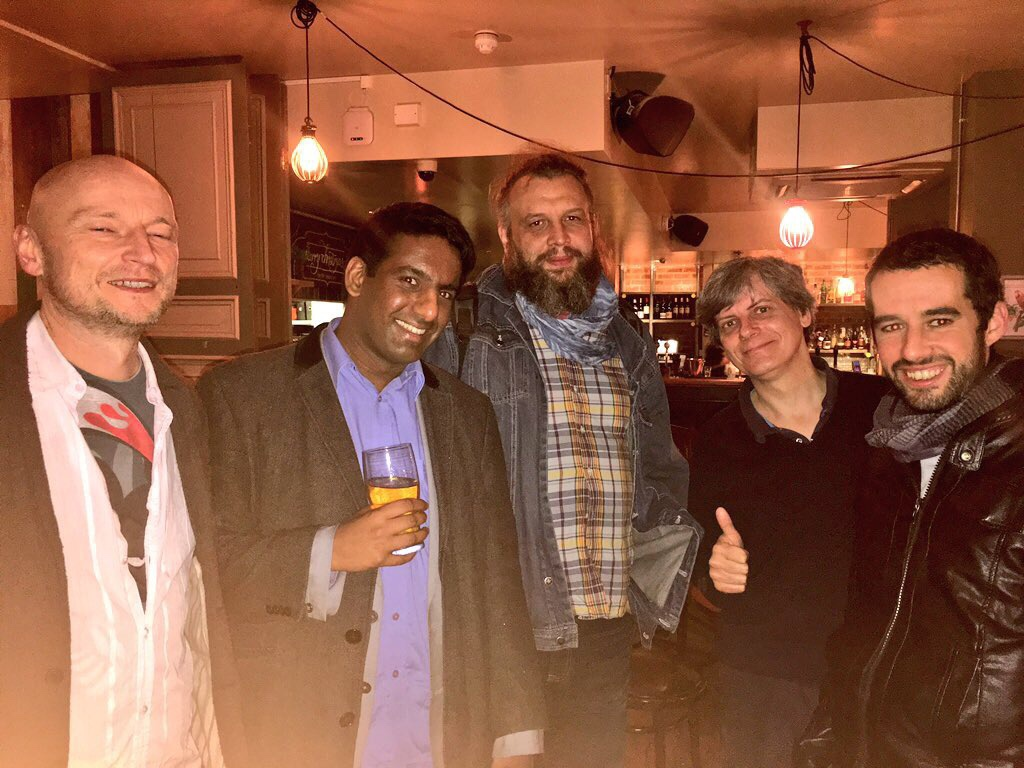
\includegraphics[scale=0.3]{img/offline/drupal_meetup_pub_london.jpg}
    \caption[London Drupal Beer and Chat]%
    {Picture at the end of a London Drupal Beer and Chat in November 2015. Retrieved \nth{2} December 2015 from \url{https://www.meetup.com/London-Drupal-Pub-Meet/photos/26552590/}. Chandeep Khosa.}
    \label{drupal-meetup-beer}
\end{figure}


\begin{figure}[H]
    \centering
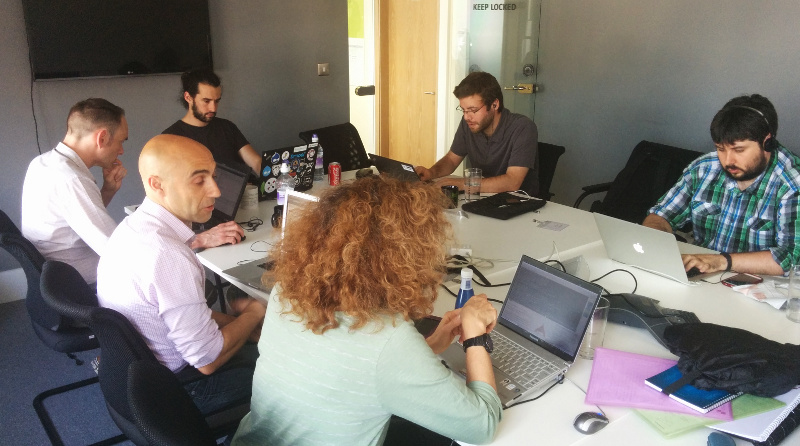
\includegraphics[scale=0.45]{img/events/drupal_coworking_day.jpeg}
    \caption[London Drupal Coworking day]%
    {Picture from a London Coworking Day in June 2014. Retrieved \nth{21} August 2014, from \url{http://www.meetup.com/London-Drupal-Coworking-Meetup/photos/22504442/}. Brian Green.}
    \label{drupal-coworking}
\end{figure}

Participation in the offline field site was more intense during specific periods, while online participation was constant. For example, after an intense period of participant observation regarding the first thematic area, participation in offline events was reduced to focus on data analysis for approximately three months, although online participation was never halted so as not to lose rapports with the community.

The participant observation in both online and offline field sites was focussed on specific areas and activities depending on the topic studied as they emerged. For example, participant observation during the study of the notion of contribution was carried out to include \textit{DrupalCamps} and at least a \textit{DrupalCon}. A similar strategy was employed regarding the second thematic area, carrying out participant observation to gain understanding of all the contribution activities studied. For example, participating in the development of \textit{contributed} and \textit{core} projects and collaborating in the organisation of local events and a \textit{DrupalCamp}. As the research was coming to an end, participant observation was significantly reduced in order to gradually leave the offline local field in London (I moved to Madrid in June 2016), as well as taking a passive role in online interactions once the data collection finished.

Overall, this method proved to be advantageous in gaining an in-depth understanding of the main topics tackled in this research, through my observations as well as other Drupalistas' actions and views: from the meanings of contribution and conflict within the Drupal community, to identifying and experiencing implicit and explicit rules that govern the self-organisational processes of contribution activities, and the ways in which the values of the community are embedded in the technical artefacts employed for collaboration. In addition, this method was beneficial to facilitate other methods. For example, to gain access to key informants and to build a rapport with them in order to persuade them to participate in semi-structured qualitative interviews, and to facilitate a more rapid evaluation of relevant materials in the documentary analysis. 

Nevertheless, participant observation can potentially introduce numerous sources of error and partiality, such as self-serving error and bias, social location skewing of the reported opinions and the directness of the report. The check list provided by \textcite{lofland2006analyzing} was employed to carry out a continuous evaluation of these sources of partiality in order to minimise them. For example, the fact that my previous experience within the Drupal community was mainly as a software developer and site builder was a potential source of partiality regarding my subjective position because of my Drupal roles (see section \ref{par:roles}). Consequently, an effort was made to have a wider understanding from the perspectives of Drupalistas with different roles during participant observation, as well as considering this during the selection of interviewees for semi-structured qualitative interviews and while carrying out documentary analysis. Another relevant potential source of partiality in cultural terms relates to the aforementioned limitations in accessing specific local communities. However, as pointed out by \textcite{kelty2008two} in his study of the cultural significance of the FLOSS phenomenon, the distributed nature of these communities makes any node a rich source of knowledge about the phenomenon itself.  Furthermore, the use of data collected through other methods, such as documentary analysis, was also employed to reduce this potential source of partiality. For example, when studying the organisational dynamics of events, blog posts regarding the organisational dynamics of equivalent events and Drupalistas' experiences of them from places as culturally diverse as Australia, the United States, India, Mexico and Nigeria were studied as part of the documentary analysis.

\subsection{Documentary analysis}
\label{subsec:documentary-analysis}

Documentary analysis is a qualitative method characterised by following a systematic procedure to review and evaluate documents with the aim of eliciting meanings and gaining understanding through interpretation \parencite{bowen2009document}.

With respect to materials found in the online field site, the vast amount of information generated by a large community such as Drupal required the definition of an initial point of collection. Although these materials could have been exclusively collected from direct sources --- for instance Drupal.org, social media channels and popular Drupal blogs --- the feed aggregator Drupal Planet\footnote{\url{https://drupal.org/planet}, accessed on \nth{9} May 2014.} was selected as such in order to cope with the extensive amount of information. Drupal Planet is a popular RSS\footnote{RSS (Really Simple Syndication) is a standard web format which allows data to be syndicated automatically.} feed within the Drupal community, whose contents are curated by Drupalistas according to certain guidelines\footnote{See \url{https://drupal.org/planet/guidelines}, accessed on 25 May 2014.}, which exclude press releases, job announcements and technical posts with little content relevant to Drupal. Since the posts at Drupal Planet are only retained for 16 weeks, a set of software scripts (see figure \ref{drupal-planet-archive}) was developed to collect and archive links to posts automatically from \nth{29} May 2013\footnote{The reason why the initial date of collection is previous to the start of the study is that previous posts were recovered from e-mail archives collected before this study.} to \nth{23} November 2016, yielding an archive of 8,613 documents relevant to this study.

\begin{figure}[H]
	\centering
	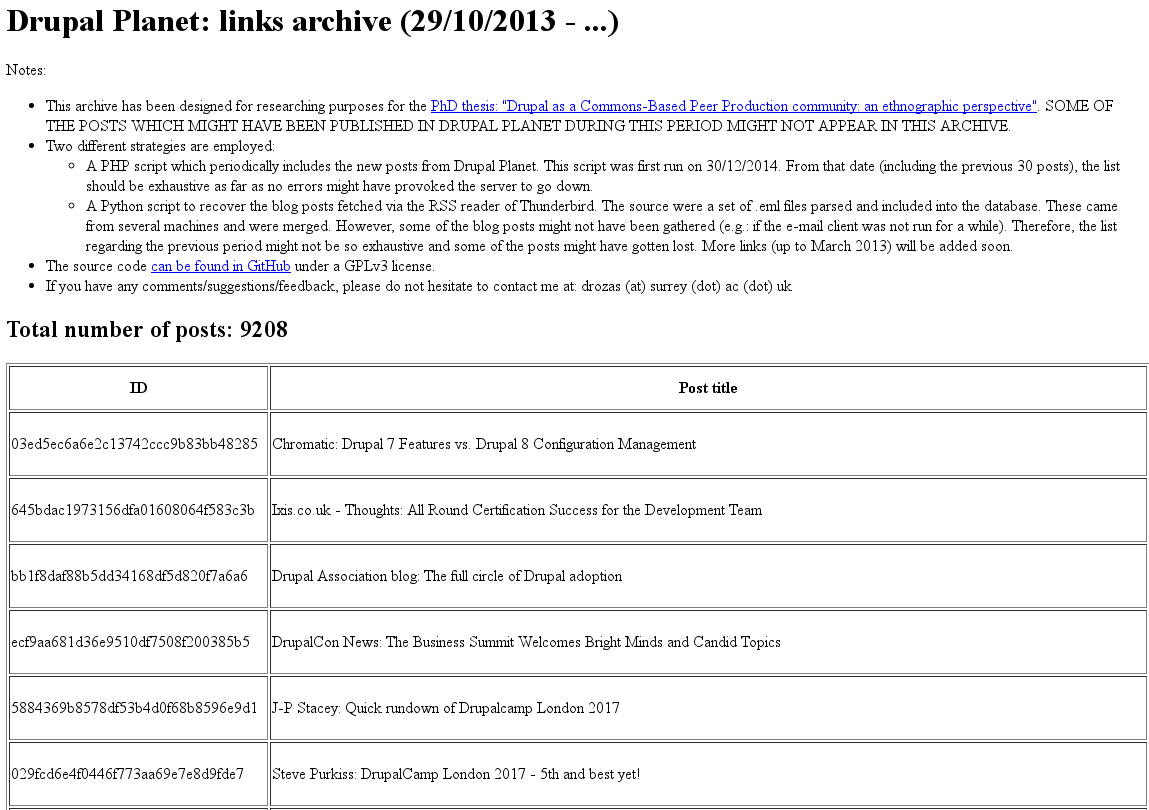
\includegraphics[scale=0.38]{img/methods/drupal_planet.png}
	\caption[Drupal Planet archive]%
    {Screenshot from the public archive of links published at Drupal Planet, accessed on \nth{8} March 2017 from \url{http://www.davidrozas.cc/lab/drupal_planet_archive.php}. The source code was released under a GPLv3 license and can be found at \url{https://github.com/drozas/drupal_planet_archive}.}
	\label{drupal-planet-archive}
\end{figure}

In addition to the materials selected from Drupal Planet, several other materials considered relevant during participant observation were included; for example, links to the discussion of an issue in a group in Drupal.org, documents mentioned during offline or online discussions, user profiles at Drupal.org, and digitised physical materials collected during offline participant observation among others. For example, the study of the first thematic area led to the need to study user profiles belonging to the main collaboration platform, as well as all the subsystems within this platform which include all secondary user profiles to the extent of my knowledge (e.g. groups.drupal.org, localise.drupal.org and assoc.drupal.org). In total, profiles from 73 users were collected using a snowball sampling until saturation was reached.

The data outcomes from this data collection method were largely diverse; for example: articles converted into PDF files, audio files from podcasts, videos from presentations, Twitter streams and collections of comments from Youtube.

With regard to documentary analysis for the notion of contribution, the inspection of materials for this stage concluded on \nth{7} October 2014, comprising a total of 3,356 documents from the archive of links. The process was carried out continuously and in parallel with participant observation: documents considered relevant were pre-coded according to the initial set of emergent themes. Table \ref{table:pilot:online-data} displays the number of materials collected during this stage, which is classified according to type of document and main theme. The percentages reflect the number of selected documents for full coding, representing 14.66\% with respect to the total of those collected in the archive of links\footnote{\label{fn:da-validity} In the analysis carried out by \textcite{drupal-planet-stats:2014:Online}, he found that around 15\% of the contents at Drupal Planet were related to the community. The meanings of ``community" differ (his criteria are more focussed on events) and this study went beyond the links provided by Drupal Planet. However, the correlation between the percentages gives a certain degree of validity to the gathered data. The intention is not to argue that this metric can be interpreted as an accurate indicator of validity of the data; however, it offered the sense that the collection of data from Drupal Planet had been carried out in the right direction.}.


    \begin{table}[h]
    \begin{footnotesize}
    \begin{tabular}{l|p{1.5cm}|p{1.5cm}|p{1.5cm}|p{1.5cm}|p{1.5cm}||p{1.5cm}|}
    \cline{2-7}
                                                          & \tiny{Contribution}    & \tiny{Economic sustainability}  & \tiny{Governance and decision-making} & \tiny{Collaboration platforms} & \tiny{Conflicts}       & \tiny{Total}                    \\ \hline
    \multicolumn{1}{|l|}{\tiny{Documents}}                       & 171             & 46              & 120                      & 32                     & 88              & 457                       \\ \hline
    \multicolumn{1}{|l|}{\tiny{Videos}}                          & 15              & 2               & 9                        & 2                      & 3               & 31                        \\ \hline
    \multicolumn{1}{|l|}{\tiny{Podcasts}}                        & 6               & 0               & 3                        & 0                      & 8               & 17                        \\ \hline
    \multicolumn{1}{|l|}{\tiny{Other datasets}\tablefootnote{\label{fn:dataset}This includes Twitter streams, collections of comments in Youtube, etc.} }                  & 3               & 0               & 5                        & 0                      & 0               & 8                         \\ \hline \hline
    \multicolumn{1}{|l|}{\tiny{Total}}                           & 195             & 48              & 137                      & 34                     & 99              & 513                       \\ \hline
    \multicolumn{1}{|l|}{\tiny{\textit{Percentage (per topic)}}} & \textit{5.57\%} & \textit{1.37\%} & \textit{3.91\%}          & \textit{0.97\%}        & \textit{2.83\%} & \textit{\textbf{14.66\%}} \\ \hline
    \end{tabular}
    \caption[Summary of materials collected for documentary analysis for the first thematic area]%
    {Summary of materials collected for documentary analysis for the first thematic area, grouped by type of document and theme.}
    \label{table:pilot:online-data}
    \end{footnotesize}
    \end{table}
    
Regarding the study of contribution activities, for the second thematic area the total number of documents from Drupal Planet yielded 8,613 (concluding on \nth{23} November 2016). Table \ref{table:ch-decent:online-data} displays the number of materials collected according to the themes discussed in section \ref{sec:data-collection} and type of document. The percentage of collected materials in total and per group was close to 10.15\% with respect to the number of links in the archive\footnote{As in the case of the previous thematic area (see footnote \ref{fn:da-validity}), this percentage was used to gain if but a limited sense of the data collection being carried out in the right direction.}.


    \begin{table}[h]
    \resizebox{\textwidth}{!}{%
    \begin{tabular}{l|p{2.3cm}|p{2.2cm}|p{2.1cm}|p{2.1cm}|p{2.1cm}||p{2.1cm}|}
    \cline{2-7}
                                                          & \textit{DrupalCon}            & \textit{DrupalCamp}            & Local events                      & \textit{Core} projects                    & \textit{Contributed} projects\tablefootnote{This includes \textit{custom} projects, since in this case the study placed the focus on the transitions between these states.}           & Total   \\ \hline
    \multicolumn{1}{|l|}{Documents}                       & 158             & 85              & 31                      & 368                     & 73              & 715                       \\ \hline
    \multicolumn{1}{|l|}{Videos}                          & 3              & 4               & 1                        & 17                      & 2               & 27 \\ \hline
    \multicolumn{1}{|l|}{Podcasts}                        & 6               & 5               & 1                        & 18                      & 0              & 30 \\ \hline
    \multicolumn{1}{|l|}{Other datasets\tablefootnote{See footnote \ref{fn:dataset}.} }                  & 14              & 12 & 10                        & 45                      & 22               & 103                         \\ \hline \hline
    \multicolumn{1}{|l|}{Total}                           & 181             & 106              & 43                      & 448                     & 97              & 875 \\ \hline
    \multicolumn{1}{|l|}{\textit{Percentage (per topic)}} & \textit{2.10\%} & \textit{1.23\%} & \textit{0.5\%}          & \textit{5.20\%}        & \textit{1.12\%} & \textit{\textbf{10.15\%}} \\ \hline
    \end{tabular}
    }
    \caption[Summary of materials collected for documentary analysis for the second thematic area]%
    {Summary of materials collected for documentary analysis for the second thematic area, grouped by type of document and theme.}
    \label{table:ch-decent:online-data}
    \end{table}
    
Overall, this method provided a relevant source of data for the analysis of the organisational dynamics of the community. For instance, to have an in-depth understanding of the historic discussions, changes and contradictions that led to the emergence of current practices and structures. It was also valuable to provide a wider perspective of the understandings of the community and its self-organisational processes at a global level, beyond participant observation. In addition, it was also helpful to facilitate tasks related to the remaining methods mentioned. For example, the inspection of certain indicators found in these materials --- such as contribution activities that are displayed on profiles and participation in Drupal events --- was useful to identify key informants to interact with during participant observation, and to verify the degree of experience, Drupal roles and areas of expertise for the selection of interviewees.

The use of Drupal Planet as an initial point for the collection of data introduced, however, several potential sources of partiality. For example, since the publication of articles in the feed is filtered by members of the community, controversial posts could potentially be excluded from the feed. A constant evaluation was performed in order to deal with this possible source of partiality. For instance, carrying out manual reviews of the issues list\footnote{\url{https://drupal.org/project/issues/content?text=&status=All&priorities=All&categories=All&version=All&component=Planet+Drupal}, accessed on \nth{20} March 2014.} in which discussions about the contents published are openly available. In addition, informal discussions were carried out with key informants responsible for the curation of these materials. Another relevant source of partiality relates to the language of the feed aggregator: Drupal Planet only allows posts in English. In order to reduce this source of partiality, an emphasis was placed on manually reviewing and including posts written in Spanish --- mainly written by Drupalistas based in South America, Spain and the United States ---  helping to partially alleviate the impact of this partiality due to the culturally subjective positions.

\subsection{Semi-structured interviews}
\label{subsec:interviews}

In addition to the unstructured and informal interviews carried out as part of the participant observation process, a total of 15 semi-structured qualitative interviews were undertaken. These interviews provided data of quality, which elicited a more precise and in-depth understanding of the life histories within the community, attitudes and motivations, subjectivities around social practices and the emergence of organisational structures, as well as the organisational dynamics and tensions of the Drupal community among other aspects. For example, the aim of the interviews carried out with regard to the study of the notion of contribution was to further understand the meanings of contribution for members of the Drupal community, its relationship with the online/offline dimension, as well as the evaluation of these activities and the representation of this value and its use on the main collaboration platform; while for the second thematic area the aim was to facilitate the uncovering of the meanings and subjectivities that surround the self-organisational processes of the contribution activities studied in the Drupal community.

The main data outcome from this data collection approach were audio files, together with transcripts that resulted from them. Additionally, full field notes were generated before and after interviews were conducted. Interviews were conducted in-person or via video/audio chat depending on the preferences of the interviewee and the feasibility of carrying out interviews in-person. Interviews in-person were carried out at the offices or homes of the interviewees, located in London and Madrid. They were undertaken in English or Spanish, depending on the choice of the interviewee.

Three interview guides were designed following the guidelines provided by \textcite{lofland2006analyzing} and \textcite{steinar1996interviews}. For example, choosing questions to create a balance of order regarding the topics to be explored to facilitate a satisfactory flow, while still allowing for flexibility to capture the interviewees' understanding of meanings with regard to their vision of their social world.

The first guide (see appendix \ref{appendix-interview-guide}) was designed with the purpose of eliciting in-depth knowledge regarding the meanings of contribution for members of the Drupal community, as well as other notions that emerged as relevant from the data collected from other methods, such as the role of affective labour in the community. The second guide (see appendix \ref{appendix-interview-guide-stage-2}) was designed to further understanding of the self-organisational processes of the contribution activities studied. The interviews started with a set of introductory questions, then progressed to the organisational processes which were relevant for each interviewee. Finally, the third guide (see appendix \ref{appendix-interview-guide-stage-3}) was tailored to elicit knowledge of the emergence and changes experienced over time in the self-organisational processes of a core initiative, which required further exploration.

Table \ref{table:interviewees-general} provides an overview of the interviewees' characteristics, including common general demographic ones, such as gender and nationality; and Drupal specific ones, such as main Drupal roles and the number of years of their Drupal.org user accounts. The characteristics were verified during the interviews, as well as previously evaluated by means of other methods --- for instance checking their profiles at Drupal.org and LinkedIn. In addition, table \ref{table:interviewees-general} provides the mode and duration of the interview.

\begin{footnotesize}

\begin{longtable}[H]{l||p{1cm}|p{1.2cm}|p{1.2cm}|p{1.4cm}|p{2cm}|p{1.2cm}|p{2cm}|p{1cm}|}
\cline{2-9}
    & \scriptsize{Duration (min.)} & \scriptsize{Mode}       & \scriptsize{Gender} & \scriptsize{Nationality} & \scriptsize{Location}             & \scriptsize{Drupal.org account years} & \scriptsize{Main role}                      & \tiny{Thematic Area}           \\ \hline \hline
\multicolumn{1}{|l||}{I\textunderscript{1}}  & 58       & in-person  & M      & USA         & London (UK)          & 7                   & Site builder and developer     & 1  \\ \hline
\multicolumn{1}{|l||}{I\textunderscript{2}}  & 70       & in-person  & M      & Mexican     & London (UK)          & 2                   & Themer and project manager     & 1  \\ \hline
\multicolumn{1}{|l||}{I\textunderscript{3}}  & 42       & in-person  & M      & Spanish     & Madrid (Spain)       & 8                   & System architect and developer & 1  \\ \hline
\multicolumn{1}{|l||}{I\textunderscript{4}}  & 113      & in-person  & M      & British     & London (UK)          & 11                  & Developer and project manager  & 1  \\ \hline
\multicolumn{1}{|l||}{I\textunderscript{5}}  & 195      & in-person  & M      & Spanish     & London (UK)          & 8                   & Developer and themer           & 2 \\ \hline
\multicolumn{1}{|l||}{I\textunderscript{6}}  & 69       & in-person  & M      & British     & London (UK)          & 9                   & Project manager                & 2 \\ \hline
\multicolumn{1}{|l||}{I\textunderscript{7}}  & 88       & video chat & M      & Spanish     & Stockholm (Sweden)   & 6                   & Developer and themer           & 2 \\ \hline
\multicolumn{1}{|l||}{I\textunderscript{8}}  & 114      & video chat & F      & USA         & Chicago (USA)        & 8                   & Developer                      & 2 \\ \hline
\multicolumn{1}{|l||}{I\textunderscript{9}}  & 80       & audio chat & M      & Austrian    & Vienna (Austria)     & 8                   & Developer                     & 2 \\ \hline
\multicolumn{1}{|l||}{I\textunderscript{10}} & 149      & video chat & M      & USA         & Chicago (USA)        & 11                  & Developer and system architect & 2 \\ \hline
\multicolumn{1}{|l||}{I\textunderscript{11}} & 86       & video chat & M      & British     & Newcastle (UK)       & 9                   & Project manager                & 2 \\ \hline
\multicolumn{1}{|l||}{I\textunderscript{12}} & 51       & video chat & F      & British     & Brighton (UK)        & 4                   & Themer                         & 2 \\ \hline
\multicolumn{1}{|l||}{I\textunderscript{13}} & 45       & video chat & M      & Finnish      & Helsinki (Finland)   & 6                   & Developer                      & 2 \\ \hline
\multicolumn{1}{|l||}{I\textunderscript{14}} & 83       & video chat & M      & Canadian    & London (Canada)      & 6                   & Developer and themer           & 2 \\ \hline
\multicolumn{1}{|l||}{I\textunderscript{15}} & 117      & video chat & M      & Danish      & Copenhagen (Denmark) & 11                  & Themer and project manager     & 2 \\ \hline
    \caption[Demographic and general interview characteristics of Drupalistas interviewed]{Demographic and general interview characteristics of Drupalistas interviewed.}
    \label{table:interviewees-general}
\end{longtable}

\end{footnotesize}

Regarding demographic characteristics, the table illustrates diversity in the nationalities of the interviewees, reflecting the global nature of the community, although, the sum of Britons and Spaniards surpasses 45\%. Another relevant characteristic that can be appreciated in this table is that most of the interviewees were male, an unfortunately unsurprising aspect since FLOSS communities are largely male-dominated \parencite{reagle2012free}. This issue was evaluated after carrying out interviews related to the first thematic area, and strategies were defined with the aim of including more female voices in subsequent interviews: 13\% of all interviews were with women, although a low number, it is closer to the 17\% of women in the Drupal community \parencite{women-in-drupal:2017:Online}.

The interviewees were chosen following a purposive sampling strategy with the aim of producing a rich range of contexts that facilitated cross-contextual comparisons \parencite[123-127]{mason2002qualitative} for each thematic area. On one hand, when studying the notion of contribution, this applied to covering a wider degree of contexts related to the notion of contribution activities according to two main criteria. Firstly, Drupal roles\footnote{See section \ref{par:roles}.}, aiming to cover each of the roles with at least two interviewees, as depicted in table \ref{table:pilot:roles-range}. Secondly, a wide range of degrees of experience, with the aim of discovering possible differences in the meanings of contributions and the outcomes of these activities according to this. To this end, the candidates were selected to fulfil different degrees of experience with an increment of three years of professional experience in Drupal\footnote{This refers to the actual years of experience working with Drupal, in contrast with the total amount of time registered at Drupal.org, which do not necessarily match. For example, I\textunderscript{1} worked with Drupal for two years starting in 2007, and reinitiated his interest in 2012.}  --- using the software as part of their main professional activity. Table \ref{table:pilot:experience-range} shows the range within which each interviewee falls.

    \begin{table}[H]
    \centering
    \begin{tabular}{l||p{1.3cm}|p{1.3cm}|p{1.3cm}|p{1.3cm}|}
    \cline{2-5}
                                                                                               & I\textunderscript{1} & I\textunderscript{2} & I\textunderscript{3} & I\textunderscript{4} \\ \hline \hline
    \multicolumn{1}{|l||}{System Architect}                                                       & \checkmark                  &                    & \checkmark                  &                   \\ \hline
    \multicolumn{1}{|l||}{Developer}                                                              & \checkmark                  &                    & \checkmark                  & \checkmark                  \\ \hline
    \multicolumn{1}{|l||}{\begin{tabular}[c]{@{}l@{}}Themer /\\ Front-end developer\end{tabular}} &                    & \checkmark                  &                    & \checkmark                  \\ \hline
    \multicolumn{1}{|l||}{Site Builder}                                                           & \checkmark                  & \checkmark                  & \checkmark                  & \checkmark                  \\ \hline
    \multicolumn{1}{|l||}{\begin{tabular}[c]{@{}l@{}}Content Editor\\ \& Manager\end{tabular}}    & \checkmark                  & \checkmark                  &                   & \checkmark                  \\ \hline
    \multicolumn{1}{|l||}{Design\slash  UX}                                                            &                    & \checkmark                  &                    & \checkmark                  \\ \hline
    \multicolumn{1}{|l||}{\begin{tabular}[c]{@{}l@{}}Project Manager\slash \\ Planner\end{tabular}}    &                    & \checkmark                  & \checkmark                  & \checkmark                  \\ \hline
    \multicolumn{1}{|l||}{Drupal Marketer}                                                        &                    &                    & \checkmark                  & \checkmark                  \\ \hline
    \end{tabular}

    \caption[Main Drupal roles of Drupalistas interviewed about the notion of contribution]{Main Drupal roles of Drupalistas interviewed about the notion of contribution.}
    \label{table:pilot:roles-range}
    \end{table}

    \begin{table}[H]
    \centering
    \begin{tabular}{l||p{1.3cm}|p{1.3cm}|p{1.3cm}|p{1.3cm}|}
    \cline{2-5}
                                                                                               & I\textunderscript{1} & I\textunderscript{2} & I\textunderscript{3} & I\textunderscript{4} \\ \hline \hline
    \multicolumn{1}{|l||}{1-3 years}   &                    & \checkmark                  &                    &                    \\ \hline
    \multicolumn{1}{|l||}{3-6 years}   & \checkmark                  &                    &                    &                    \\ \hline
    \multicolumn{1}{|l||}{6-9 years}   &                    &                    & \checkmark                  &                    \\ \hline
    \multicolumn{1}{|l||}{10-12 years} &                    &                    &                    & \checkmark                  \\ \hline
    \end{tabular}
    \caption[Ranges of experience of Drupalistas interviewed about the notion of contribution]{Ranges of experience of Drupalistas interviewed about the notion of contribution.}
    \label{table:pilot:experience-range}
    \end{table}

On the other hand, for interviews regarding the study of the self-organisational processes of the contribution activities studied, the  interviewees were selected according to the prominence of their role in the coordination and understanding of the inner workings of the processes of these activities, which allowed for a wide degree of domains of knowledge. For example, being gatekeepers of certain peer-reviewing processes, such as in \textit{custom} projects to become \textit{contributed} ones, or the selection of presentations in a \textit{DrupalCon}; having an in-depth knowledge of the changes experienced over time in the self-organisational processes; or being significant organisers of local events and \textit{DrupalCamps}. The aim was to cover each contribution activity with at least four interviewees. Table \ref{table:decent:contexts-rage} shows the range within which each interviewee falls, having fulfilled this goal. In addition, interviewees I\textunderscript{11}-I\textunderscript{15} were selected on the basis of providing a rich set of contexts with respect to the changes experienced over time in a core initiative: from one of the pioneers of the initiative, to Drupalistas who joined it in subsequent years and went on to lead its technical direction. Two main reasons explain why a specific stage was necessary for this case. Firstly, core processes have a higher degree of organisational complexity regarding their self-organisational processes, requiring deeper immersion overall. Secondly, this specific initiative was led by themers (see section \ref{par:roles}), a role significantly different to those I have held as a Drupalista. Hence, this required my immersion technically, as well as more intensively in the initiative in order to better understand the dynamics behind it and to gain access to key members.

\begin{longtable}{p{1.5cm}||p{0.5cm}|p{0.5cm}|p{0.5cm}|p{0.5cm}|p{0.5cm}|p{0.5cm}|p{0.5cm}|p{0.5cm}|p{0.5cm}|p{0.5cm}|p{0.5cm}|}
\cline{2-12}
                                  & I\textunderscript{5} & I\textunderscript{6} & I\textunderscript{7} & I\textunderscript{8} & I\textunderscript{9} & I\textunderscript{10} & I\textunderscript{11} & I\textunderscript{12} & I\textunderscript{13} & I\textunderscript{14} & I\textunderscript{15}\\ \hline \hline
\multicolumn{1}{|l||}{Local events}			& \checkmark  & \checkmark  & \checkmark & 			  & 		   & 			& \checkmark & & & &\\ \hline
\multicolumn{1}{|l||}{\textit{DrupalCamps}}    		& \checkmark  & \checkmark  & \checkmark & \checkmark & \checkmark & \checkmark & \checkmark & & & & \\ \hline
\multicolumn{1}{|l||}{\textit{DrupalCons}}     		& \checkmark  &  			& \checkmark & \checkmark & 		   & \checkmark & \checkmark & & & & \\ \hline
\multicolumn{1}{|l||}{\textit{Core} projects}  	& \checkmark  & 			& \checkmark & \checkmark & \checkmark & \checkmark & & \checkmark & \checkmark & \checkmark & \checkmark \\ \hline
\multicolumn{1}{|l||}{\textit{Contributed} projects\footnote{This includes the discussion about \textit{custom} projects becoming \textit{contributed} ones.}} 	& \checkmark  &  			& \checkmark & \checkmark & \checkmark & \checkmark & & & & & \\ \hline
\caption[Domains of knowledge of the interviewees with regard to the contribution activities studied]{Domains of knowledge of the interviewees with regard to the contribution activities studied.}
\label{table:decent:contexts-rage}
\end{longtable}


A relevant potential source of partiality considered when drawing on this method referred to social desirability. For example, since contributing back to the community is seen in CBPP communities as a source of social capital, the interviewees might over-represent their contributions when asked about them, or they might consider that the types of contribution they undertake are more relevant than those of other Drupalistas. In order to reduce this source of partiality, interviewing techniques were employed --- for instance, asking first about how it is possible for people to contribute, rather than directly how \textit{they} do it --- in combination with an evaluation by means of other methods --- for instance, inspecting their contributions via documentary analysis. Another potential source of partiality, related to purposive sampling, can be seen in my location as an ethnographer in the UK and my previous experience in the Spanish community. However, the use of online interviews alleviated the potential impact of this source of partiality, carrying out interviews by video/audio chat in cases where wider degrees of contexts were necessary.

\subsection{Organising and analysing the data}
\label{organising-caqdas}

In order to manage the considerable amount of data collected and generated during this study, CAQDAS\footnote{Concretely, the proprietary CAQDAS package NVivo 10 (\url{http://www.qsrinternational.com/products_nvivo.aspx}, accessed on \nth{12} February 2014) was employed. An evaluation to compare different CAQDAS packages was carried out at the beginning of the study, including FLOSS CAQDAS packages, such as RQDA (\url{http://rqda.r-forge.r-project.org/}, accessed on \nth{12} February 2014), LibreQDA (\url{http://www.libreqda.edu.uy/}, accessed on \nth{12} February 2014) or WeftQDA (\url{https://www.webqda.com/}, accessed on \nth{12} February 2014), as well as other proprietary options \parencite{caqdas2009}. Despite the emphasis placed throughout this study on giving priority to the use of FLOSS tools, CAQDAS was the exception. It was concluded that FLOSS alternatives did not fulfil some of the requirements which would facilitate data collection, organisation and analysis for this research; or in cases where requirements were partially fulfilled, they were found not to be stable enough. For example, FLOSS tools offering equivalent functionalities to those provided by NCapture --- a browser plugin which allows users to collect websites easily, Twitter datasets and Youtube comments among others --- did not exist at the time of the evaluation to the best of my knowledge.} (Computer Assisted Qualitative Data AnalysiS) software was employed to facilitate the archiving, organisation and analysis of the data. The use of this tool facilitated several tasks, such as the creation of transcripts, the coding and analysis of the codes. Figure \ref{model-merged} depicts, for example, the use of CAQDAS software for the creation of models developing from the main concepts of Activity Theory, and the emergence of codes related to ``mostly-offline" contribution activities.

\begin{figure}[H]
	\centering
	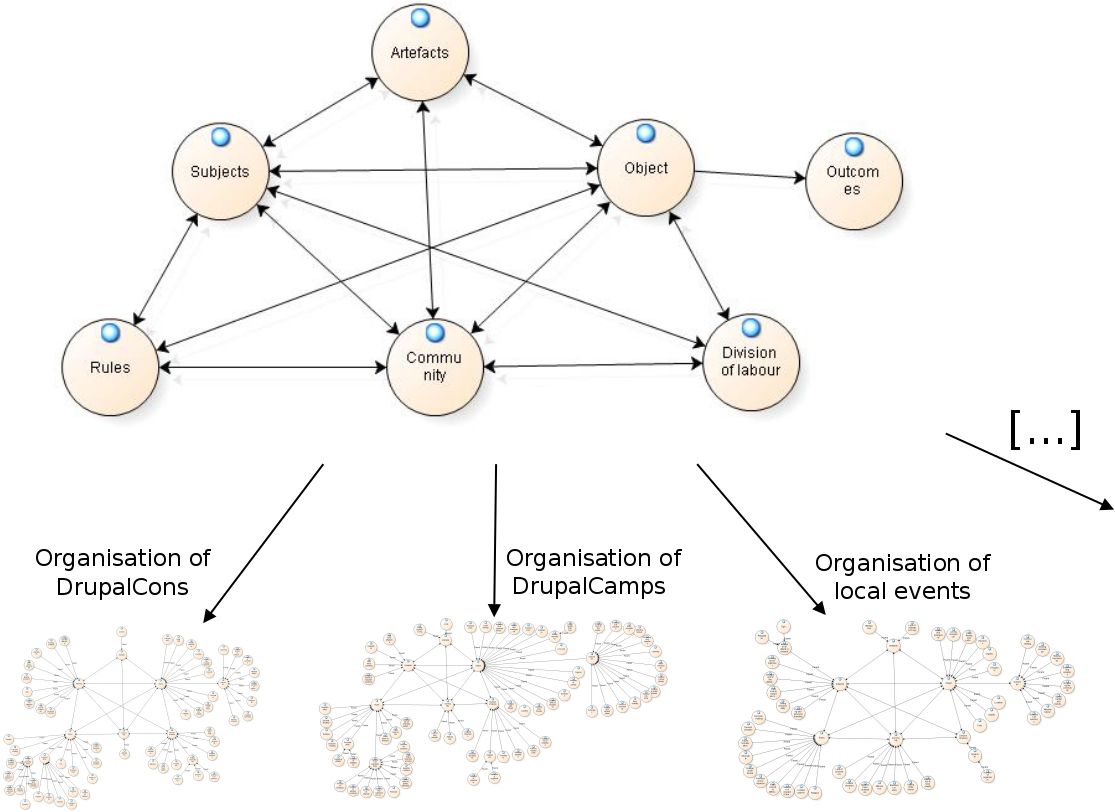
\includegraphics[scale=0.38]{./diagrams/models_merged_ta2.png}
	\caption[Emergent categories conceptualised through the general model of Activity Theory]{General model of Activity Theory and emerging categories during a third major iteration in the analysis of contribution activities of the second thematic area.}
	\label{model-merged}
\end{figure}

In addition, the large amount of data generated and collected during the undertaking of this research required a strategy to store and manage this data, including the automatic creation of backups, maintaining a revision control system or securely accessing these data from several locations and devices. External cloud computing services provide optimal means to easily fulfil these requirements, however, they come at a cost: data is stored on third-party servers. Hence, at the beginning of the study, several possible solutions were evaluated on the basis of the degree of security, and a two-layer strategy was designed, according to the size of the files.

GitHub\footnote{\url{https://github.com/}, accessed on \nth{10} March 2014.} was chosen as the primary repository. Github is a service that provides Git\footnote{See section \ref{subsec:floss-tools}.} repositories with all the advantages of the cloud, and it is widely used by FLOSS communities. The security policy of GitHub is considerably strong, including encryption during transmission, auditions on operational security, and biometric measures for physical security, \parencite{github-security2014}. The dedication to security was the reason for selecting this specific platform, and a private repository was created to store most of the data --- field notes, transcripts and materials from documentary analysis. Nonetheless, GitHub limits the size of files to 100MB. Hence, files exceeding that size --- concretely audio recordings and the main CAQDAS file ---  were stored in a secondary repository. In this case, the service chosen was Dropbox\footnote{\url{https://www.dropbox.com}, accessed on \nth{9} July 2014.}. Dropbox is a cloud-computing file hosting service, whose security policy was also evaluated, concluding that the degree of security was equivalent to that offered by GitHub\footnote{Similar security measures to those employed by GitHub are described on the company's website \parencite{dropbox-security2014}, although with a lower level of technical detail.}.

Security announcements from both services were followed in order to immediately remove the data in case the services were compromised at any point. In addition, once the study concluded, all files stored in any third-party services were removed and registered with the University of Surrey and will be hosted and retained for a period of at least ten years, following the regulations from the University's data management policy \parencite{uniS-data-management:2017:Online}.

\section{Ethical considerations}
\label{par:ethical-gen}

In order to ensure this study fulfils the ethical principles described by the University of Surrey, an evaluation was undertaken as to whether this study should be referred to the University Ethical Committee to seek an ethical review. This research did not fall into any of the categories\footnote{Appendix \ref{unis_ethics} provides a more extensive overview of these categories and the reasons why it was considered this study did not fall into any of them.} described by the Ethical Principles \& Procedures for Teaching and Research \parencite[4-5]{UEC2013} and, hence, it was concluded that it was unnecessary. Nevertheless, the study was carried out considering the recommendations at all times. For example, when the processing of personal data required the personal consent of the participant, such as in the case of qualitative interviews, the process was carried out according to the suggested Data Protection Act (1998). In addition to the guidelines provided by the University of Surrey, the ``Recommendations from the Association of Internet Researchers Ethics Working Committee" \parencite{markham2012} were evaluated and constantly considered during the course of this study. This document provides a set of guidelines to facilitate the process of ethical assessment in the field of Internet studies, as well as a set of common questions to help the researcher to raise ethical considerations.

The ethnographic approach followed in this study required constant assessment of the possibility of new ethical issues arising during its course. Hence, the strategy consisted of keeping an iterative assessment employing these guidelines, and when new issues were discovered, actions were designed and implemented.

For example, regarding participant observation, a fundamental ethical consideration was related to the type of access. Participant observation was carried out in a ``partially overt" way: aiming to be undertaken in ``the most overt" way possible, but being aware of the limitations. The role cannot be classified as a completely known observer one since it was impractical, and probably impossible, to make all participants aware of this during the undertaking of the process. Instead, strategies were designed and followed to carry out participant observation in an ``as overt as possible" manner in both online and offline domains of the field site.

For instance, when I was asked about my motivation to participate in an event while carrying out participant observation in the offline field site, I always provided the explanation that I was a Drupalista who was currently studying the Drupal community for my PhD research. During the initial events attended, for example, an explanation based on the notes depicted in figure \ref{intro_draft} was provided. Over the course of the study, however, Drupalistas became more aware of my role as a researcher, more significantly at local events. Indeed, I was often introduced to other Drupalistas as ``the guy who is doing a PhD about the Drupal community". 

\begin{figure}[H]
	\centering
	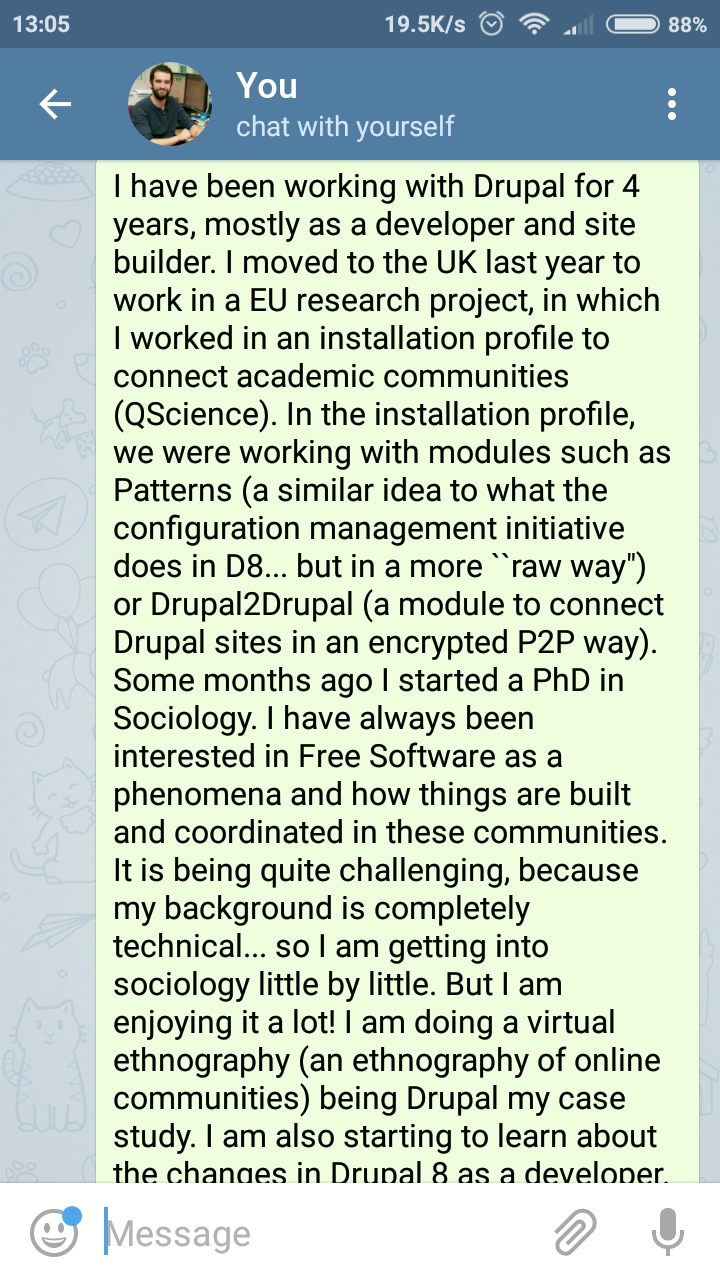
\includegraphics[scale=0.3]{img/methods/notes_telegram_introduction.png}
	\caption[Notes introducing my role as researcher and Drupalista]{Notes depicting an introduction of my role as researcher and Drupalista prepared before attending an event for the first time.}
	\label{intro_draft}
\end{figure}

Additionally, an effort was made to expose this study, and hence my role as researcher, to the global community to the highest degree possible. For example, presenting the first set of findings from this study in local events, \textit{DrupalCamps} and a \textit{DrupalCon}\footnote{See sections on non-academic events at \url{http://davidrozas.cc/presentations} to find more details related to my participation as speaker, as well as a list of reviews and opinions from Drupalistas.}, and participating in interviews in Drupal channels, such as a Drupal podcast\footnote{See \url{https://www.drupaleasy.com/podcast/2015/10/drupaleasy-podcast-163-drupal-potato-david-rozas-open-source-contributing}.} or videos regarding Drupal events\footnote{See \url{https://www.youtube.com/watch?v=DrbJ9xwSstE}.}. Notwithstanding, the role cannot be qualified as that of a completely known observer, since some attendees were not aware of my role as observer, especially while participating in large international events, such as \textit{DrupalCons}, with thousands of attendees. 

Regarding online participation, strategies were also designed and followed with the aim of carrying out observations in an ``as overt as possible" manner. For example, descriptions explaining my role as researcher were posted on the digital platforms employed by the community to facilitate the organisation of these events: from Drupal.org (see figure  \ref{intro_dorg}), to profiles on specific sites created for \textit{DrupalCamp} and \textit{DrupalCons}\footnote{See \url{https://amsterdam2014.drupal.org/users/drozas}, accessed on \nth{5} November 2014,  for an example.}  or on external platforms employed in the organisation of local events\footnote{See \url{http://www.meetup.com/London-Drupal-Pub-Meet/members/122334662/}, accessed on \nth{5} November 2014, for an example.}. In addition, the previously discussed efforts to expose this study were also valuable when carrying out this process in ``the most overt" way possible, although, as in the case of the offline field site, it has to be understood as ``partially overt".

\begin{figure}[H]
	\centering
	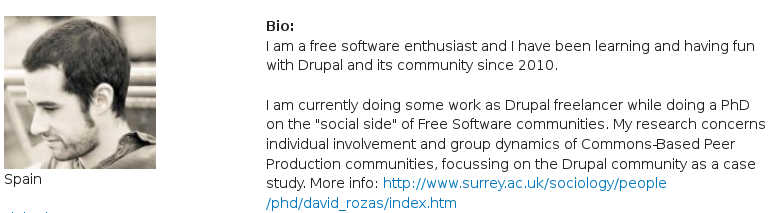
\includegraphics[scale=0.53]{img/methods/d_org_my_profile.png}
	\caption[Introduction in profile at Drupal.org]%
    {Introduction in my profile Drupal.org, version updated on November 2014 to include a link to my official profile at the University of Surrey, accessed on \nth{7} March 2015 from \url{https://www.drupal.org/u/drozas}.}
	\label{intro_dorg}
\end{figure}

Another example of relevant ethical considerations, related in this case to documentary analysis, arose with respect to the use of materials quoted in this thesis. In accordance with the principles of FLOSS culture, most of the materials created by Drupalistas are under Creative Commons licenses\footnote{This thesis was always aimed to be published under a compatible Creative Commons License. The implications of this type of licenses for publication in academic journals --- for instance, a possible limitation regarding publishing only in Open Access ones --- were, however, explored and queried to the Copyright and Digital Resources Advisor in the University's Library. For instance, it was clarified that ``The Copyright and Rights in Performances (Quotation and Parody) Regulations 2014" (\url{http://jiscleg.al/quotation}, accessed on \nth{21} October 2014) which came into force in October 2014 \emph{``permits a short quotation that is necessary and relevant in an essay or academic paper"}, allowing the publication of derivative works in non-open access journals.}. For example, the contents published in Drupal.org are under an Attribution-Share Alike 2.0 Creative Commons license\footnote{\url{https://creativecommons.org/licenses/by-sa/2.0/}, accessed on \nth{15} April 2014.}, allowing the reuse of these materials. Nevertheless, for materials collected in a private sphere --- such as private conversations in Twitter and private e-mails --- explicit permission was requested electronically to use them. For these cases the materials were additionally anonymised, as previously depicted by figure \ref{telegram_interaction}. When materials were noted as sensitive by Drupalistas --- such as the specific technical criteria to determine the ``not a spammer" role discussed in section \ref{par:roles} --- the information was omitted.

Finally, for the case of semi-structured qualitative interviews, consent forms (see appendices \ref{appendix-consent-form}, \ref{appendix-consent-form-stage-2} and \ref{appendix-consent-form-stage-3}) were prepared before conducting them. The processing and use of personal data --- such as first and last name, Drupal username and employment situation and company --- of the interviewees required their personal consent \parencite{UEC2013}, and the interviews were electronically recorded for further analysis. The purpose of this document was to ensure that the participant was aware of and properly understood the purpose of the research, as well as to clearly inform them that all data collected would be processed and anoymised in the strictest confidence. Two different strategies were designed for agreement depending on the medium employed for the interview. For in-person interviews, two copies of the consent form were presented to the participant to be signed: one was delivered to the participant and the other was collected by the researcher. Regarding interviews conducted via video/audio chat, the consent was obtained ``on tape" and recorded at the beginning of the interview. The standard form wording\footnote{Concretely: \emph{``Do you understand and consent that all personal data will be held and processed in the strictest confidence, and in accordance with the Data Protection Act (1998)?"}} described in \textcite{UEC2013} was read, and the interviewee was requested to agree in order to start the interview. 

\section{Conclusion}

Throughout this chapter the most determinant aspects regarding the methodological approach taken for this study were extensively discussed. The ethnographic approach followed enabled an in-depth exploration of the organisational dynamics of a global, large and well-known case study of Commons-Based Peer Production. The decision to follow the ethnographic approach detailed above was made on the basis of the nature of the research questions which required, firstly, an inductive approach which assumed that the topics would emerge from the process of data analysis rather than vice versa; and, secondly, a methodological approach which would acknowledge the need to understand these topics from within the community.

To this end, a multi-modal approach was followed regarding data collection, in which data collected and generated from participant observation, documentary analysis and semi-structured qualitative interviews were integrated and combined to further the analysis of the data in a way that each method informed all others. For example, drawing on documentary analysis to develop a broader view of the observations generated in the field site, and the recruitment of candidates to interview more formally by means of gaining access through participant observation, as it was extensively discussed in the second section of this chapter. Finally, this chapter concluded with an account of the most relevant ethical aspects considered during the course of the study.

The next chapter marks the beginning of the presentation of findings for this thesis focussing on the notion of contribution, a fundamental concept that underpins the study of the self-organisational aspects surrounding the contribution activities explored in proceeding chapters.